\documentclass[12pt]{article}

\usepackage{answers}
\usepackage{setspace}
\usepackage{graphicx}
\usepackage{enumitem}
\usepackage{multicol}
\usepackage{mathrsfs}
\usepackage[margin=1in]{geometry} 
\usepackage{amsmath,amsthm,amssymb}
\usepackage{pgfplots}
\usepackage{listings}
\pgfplotsset{compat=1.15}
\usepgfplotslibrary{fillbetween}
 
\newcommand{\N}{\mathbb{N}}
\newcommand{\Z}{\mathbb{Z}}
\newcommand{\C}{\mathbb{C}}
\newcommand{\R}{\mathbb{R}}

\DeclareMathOperator{\sech}{sech}
\DeclareMathOperator{\csch}{csch}
 
\newenvironment{theorem}[2][Theorem]{\begin{trivlist}
\item[\hskip \labelsep {\bfseries #1}\hskip \labelsep {\bfseries #2.}]}{\end{trivlist}}
\newenvironment{definition}[2][Definition]{\begin{trivlist}
\item[\hskip \labelsep {\bfseries #1}\hskip \labelsep {\bfseries #2.}]}{\end{trivlist}}
\newenvironment{proposition}[2][Proposition]{\begin{trivlist}
\item[\hskip \labelsep {\bfseries #1}\hskip \labelsep {\bfseries #2.}]}{\end{trivlist}}
\newenvironment{lemma}[2][Lemma]{\begin{trivlist}
\item[\hskip \labelsep {\bfseries #1}\hskip \labelsep {\bfseries #2.}]}{\end{trivlist}}
\newenvironment{exercise}[2][Exercise]{\begin{trivlist}
\item[\hskip \labelsep {\bfseries #1}\hskip \labelsep {\bfseries #2.}]}{\end{trivlist}}
\newenvironment{solution}[2][Solution]{\begin{trivlist}
\item[\hskip \labelsep {\bfseries #1}]}{\end{trivlist}}
\newenvironment{problem}[2][Problem]{\begin{trivlist}
\item[\hskip \labelsep {\bfseries #1}\hskip \labelsep {\bfseries #2.}]}{\end{trivlist}}
\newenvironment{question}[2][Question]{\begin{trivlist}
\item[\hskip \labelsep {\bfseries #1}\hskip \labelsep {\bfseries #2.}]}{\end{trivlist}}
\newenvironment{corollary}[2][Corollary]{\begin{trivlist}
\item[\hskip \labelsep {\bfseries #1}\hskip \labelsep {\bfseries #2.}]}{\end{trivlist}}
 
\begin{document}
 
% --------------------------------------------------------------
%                         Start here
% --------------------------------------------------------------
 
\title{Problem Set 5}%replace with the appropriate homework number
\author{Basil R. Yap\\ %replace with your name
50.021 Artificial Intelligence - Term 8} %if necessary, replace with your course title
\date{June 19, 2018}
\maketitle
%Below is an example of the problem environment

\section{Theory Component}
% Question 1
\begin{figure}[h!]
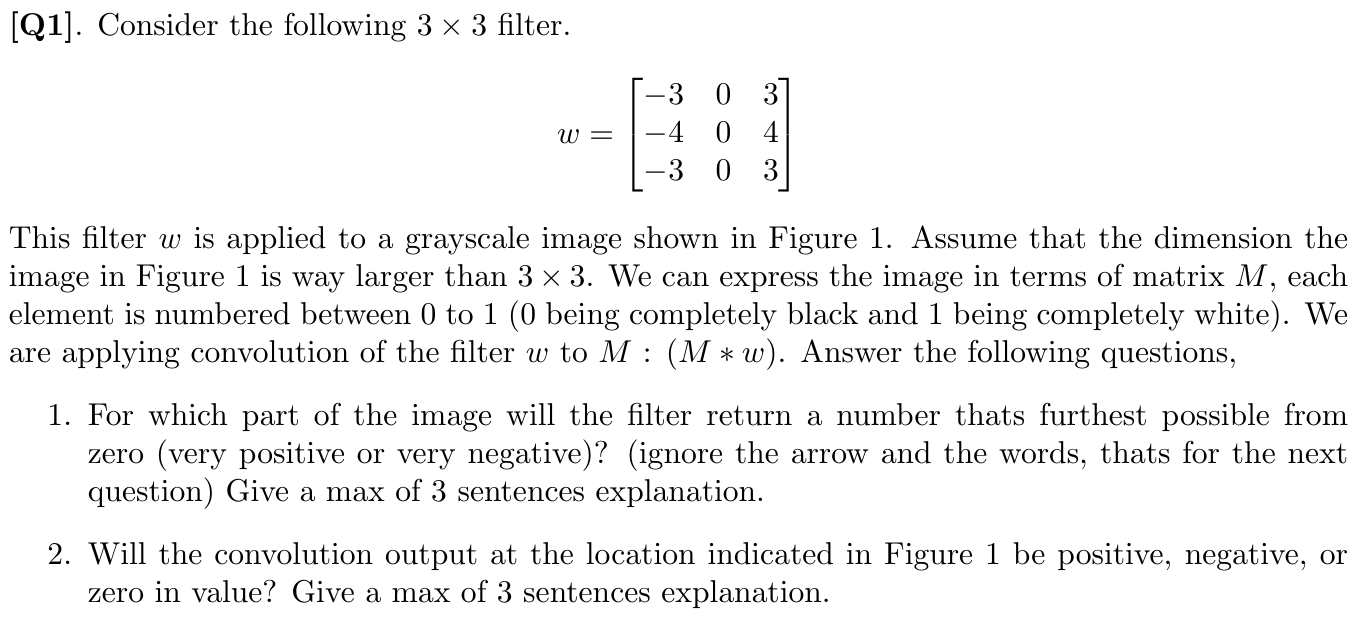
\includegraphics[width=\linewidth]{./assets/201806300414.png}
\end{figure}
\pagebreak
\begin{figure}[h!]
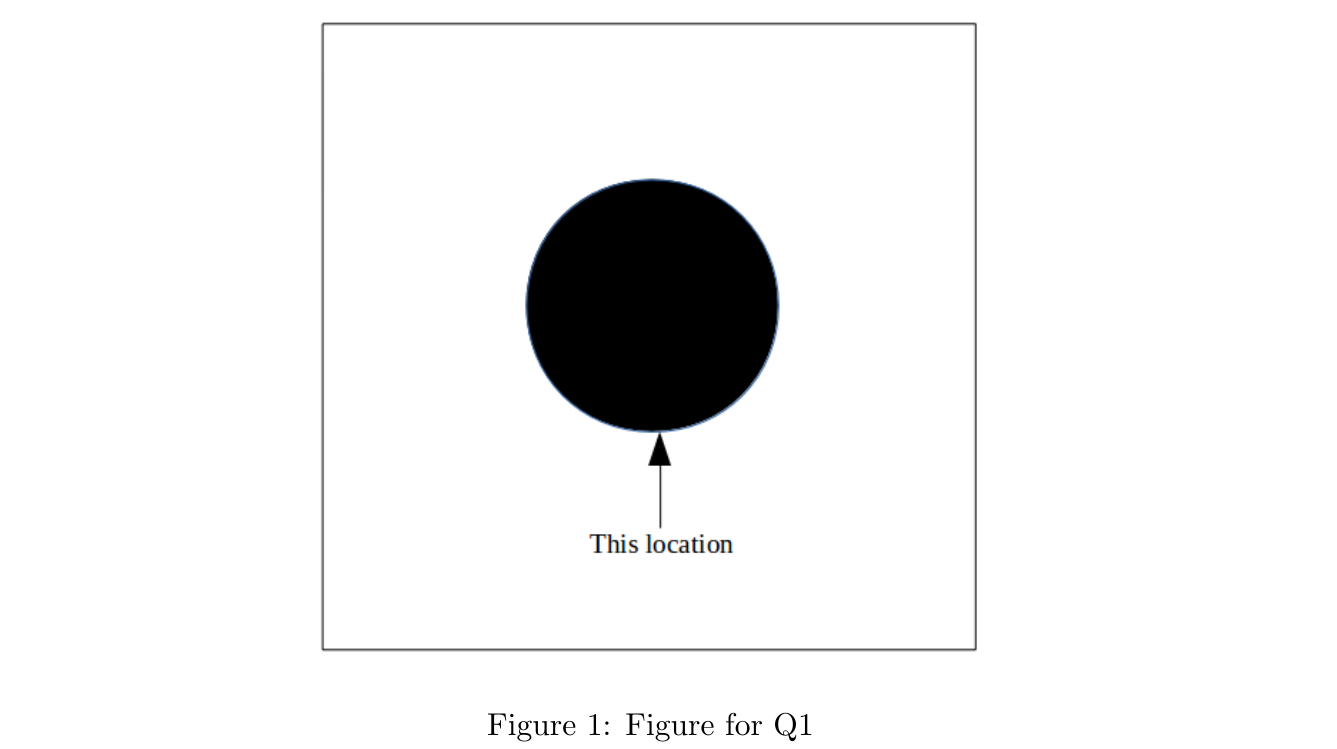
\includegraphics[width=\linewidth]{./assets/201806300418.png}
\end{figure}

\begin{solution}{}~
\begin{enumerate}
\item The parts with the largest magnitude from zero lies at the rightmost and leftmost parts of the circle. The rightmost having the most negative value, while the leftmost has the most positive value.
\item That location will have zero in value, as the values at that point would have values which are symmetrical along the columns of the filter. The filter, having equal negative and positive multiplier, will result in a zero sum when convoluted.
\end{enumerate}
\end{solution}

% Question 2
\begin{figure}[h!]
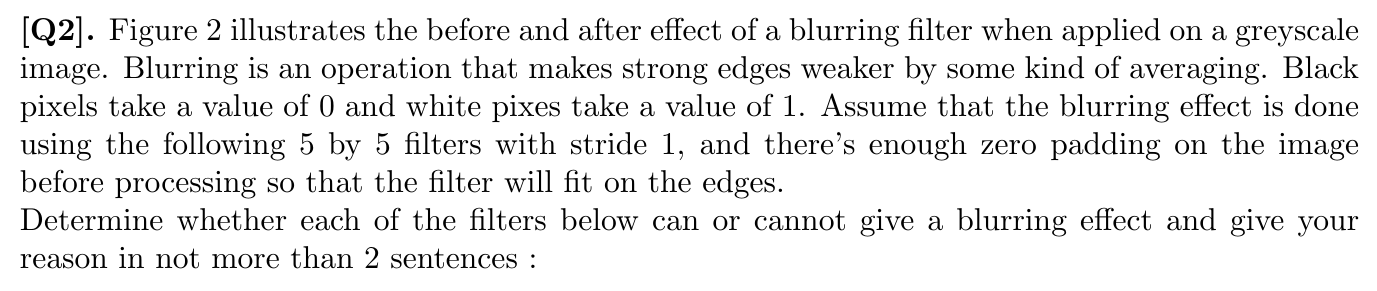
\includegraphics[width=\linewidth]{./assets/201806300415.png}
\end{figure}
\begin{figure}[h!]
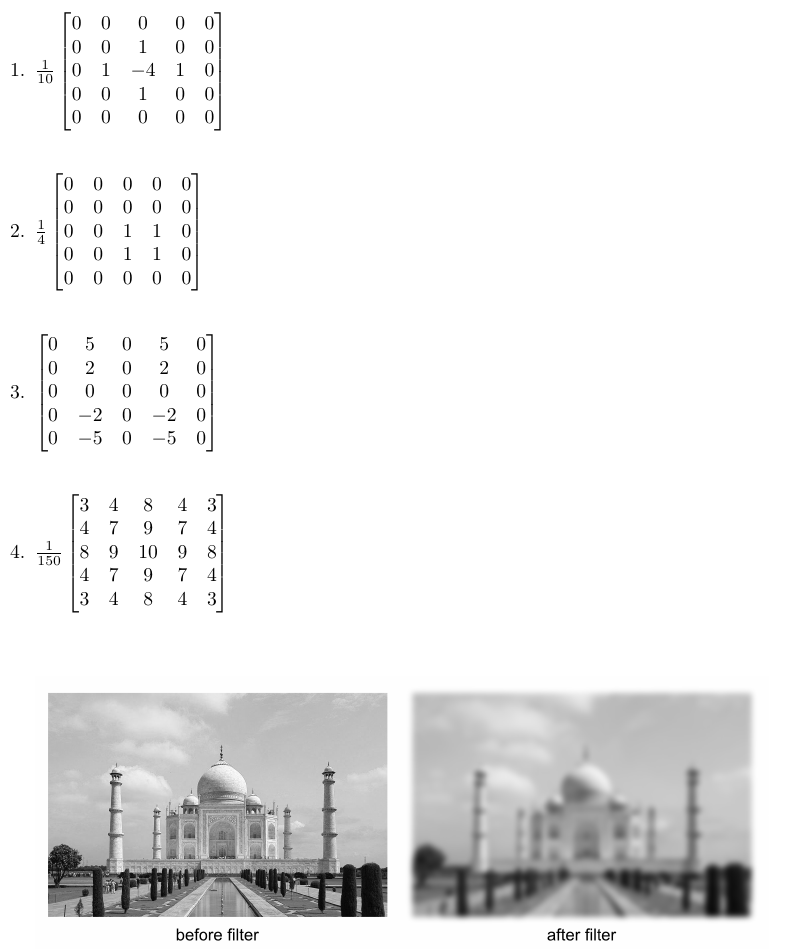
\includegraphics[width=\linewidth]{./assets/201806300416.png}
\end{figure}
\pagebreak
\begin{solution}{}~
\begin{enumerate}
\item Cannot result in blurring effect. This filter takes a huge weight for the central pixel in relation to surrounding pixels, preserving the overall contrast of the image but inverting its colour. This filter may result in sharper contrast than the original image.
\item Can result in blurring effect. This filter averages the value of the central pixel indiscriminately with other pixels from the bottom right region. Blurring will occur toward the bottom and right side of the image.
\item Cannot result in blurring effect. Given a vertical edge, the filter has a high likelihood of returning zero or close to zero in value. The low value regions will create huge contrast and not contribute to a blurring effect. This filter is used to detect horizontal edges while downsampling the resolution of the image.
\item Can result in blurring effect. This filter averages the value of the central pixel with all other pixels in the filter, but with emphasis on the central pixel and the pixels surrounding it. 
\end{enumerate}
\end{solution}


% Question 3
\begin{figure}[h!]
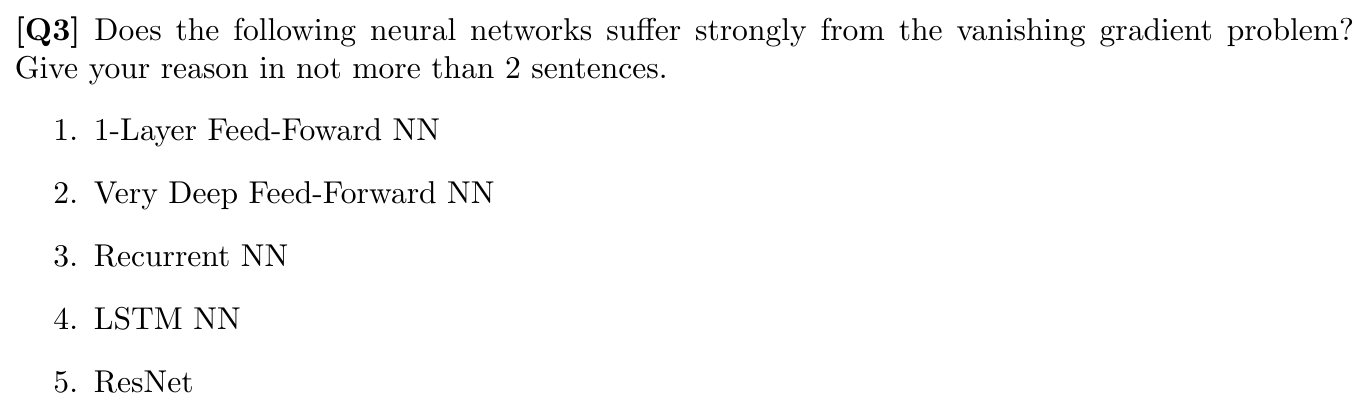
\includegraphics[width=\linewidth]{./assets/201806300417.png}
\end{figure}

\begin{solution}{}~
\begin{enumerate}
\item Does not suffer greatly from the vanishing gradient problem. Backpropagation only occurs back one layer.
\item Suffers greatly from vanishing gradient problem. With a significant number of layers, the changes to the gradient of earlier layers are greatly diminished.
\item Suffers greatly from vanishing gradient problem. Due to the time component of the RNN, backpropagation through time has more parameters to consider at each step and results in the gradients of earlier layers to change less.
\item Does not suffer greatly from the vanishing gradient problem. Due to the presence of the forget gate in LSTM, the change in gradient remains constant in recurrence and will not vanish as it propagates back to the earlier layers. 
\item Does not suffer greatly from the vanishing gradient problem. With the identity shortcut connection, the gradients of earlier layers would be less likely to be heavily diminished during backpropagation through many layers.
\end{enumerate}
\end{solution}

\section{Coding Component}

\lstinputlisting[language=Python]{pset5.py}

\end{document}
